Um den Effekt der Implementierung der nebenläufigen Architektur quantitativ analysieren zu können, werden einige Szenarien in der Blocklib definiert. Diese Szenarien werden werden dann in einem Stand vor der Integration der nebenläufigen Architektur und einem Stand danach durchlaufen. Da die Blocklib unter Nutzung des Versionsverwaltungstools Git~\cite{Chacon2014} entwickelt wird, lassen sich sogenannte Hashes angeben, die genau definieren, welche Versionen der Blocklib für die Performanceanalyse genutzt werden. Diese Hashes werden auch Revisionsnummern genannt. Die genutzten Hashes sind in Tabelle~\ref{tab:perfHash} aufgelistet.
\begin{table}
	\centering
	\begin{tabular}{ll}
		\toprule
		Stand & Hash / Revisionsnummer \\
		\midrule
		Nebenläufige Architektur & \texttt{110d0f9c227cb85d131c4f04fdf83b07ee218f39}\\
		Ursprüngliche Architektur & \texttt{d392933e558a9864ad71e7e3ccf8561f2c16b1b3} \\
		\bottomrule
	\end{tabular}
	\caption{Revisionsnummern des Versionsverwaltungstools der Blocklib, die für die Performanceanalyse genutzt werden.}\label{tab:perfHash}
\end{table}

Insgesamt werden fünf verschiedene Szenarien betrachtet. In allen Szenarien werden die folgenden Messwerte ausgewertet: \si{\fps}, Auslastung des Prozessors (CPU), Auslastung der Grafikkarte (GPU) und Speichernutzung. In jedem Szenario läuft die Blocklib für \SI{60}{\second}. Ausschlaggebend hierfür ist die durch Java mit der Methode \code{System.currentTimeMillis()} bereitgestellte Zeit. Der Code, der für die Ausführung der Szenarien benötigt wird, ist der Masterarbeit beigelegt.
\todo{Messwekzeuge nennen}
\todo{Hardware nennen}

\subsubsection{Szenario 1: Hexagon}
Um den Effekt der nebenläufigen Architektur möglichst zu isolieren, werden in den Szenarien 1 und 2 keine zufällig generierten Welten genutzt. Stattdessen werden die Blöcke nach einem festgelegten Muster gesetzt.

\begin{figure}
	\centering
	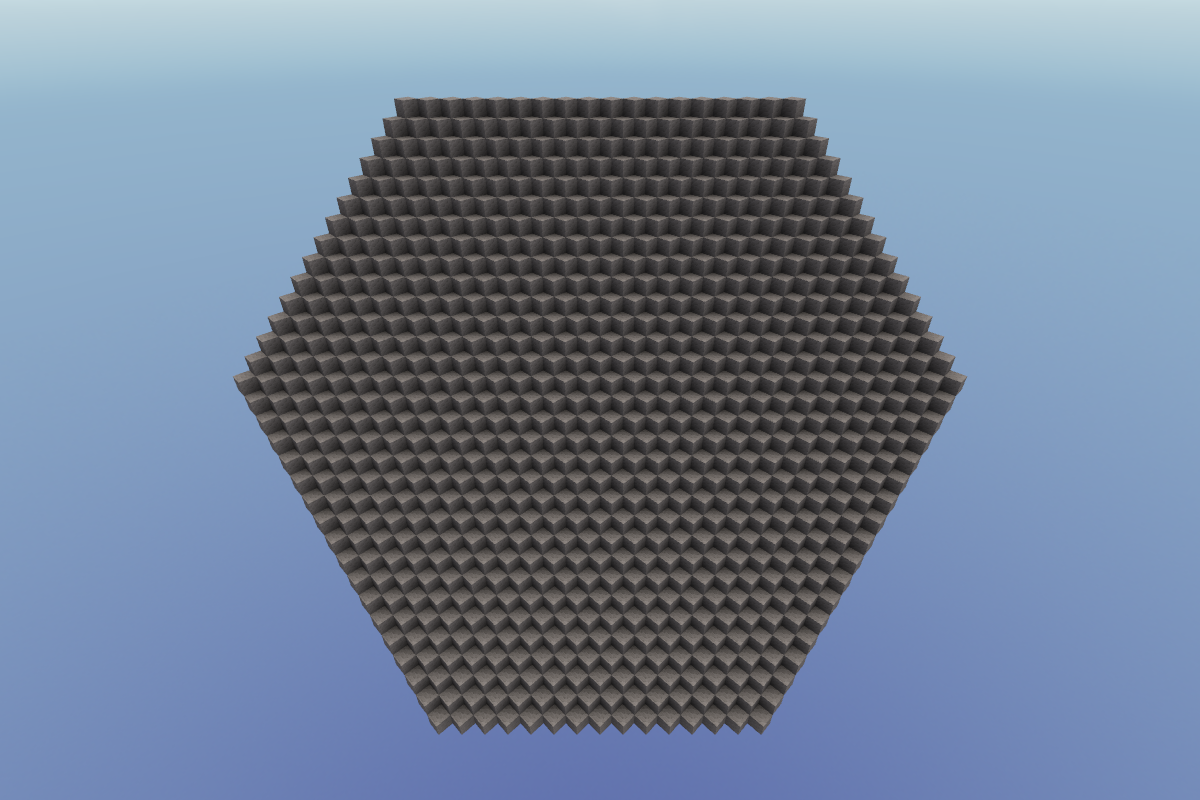
\includegraphics[width=.8\textwidth]{fps-hexagon.png}
	\caption{Screenshot der Blockformation in Szenario 1. Die Blöcke bilden ein stilisiertes Hexagon. Es ist \emph{nicht} gleichseitig. Die Formation ermöglicht den Blick auf je drei Seiten jedes Blocks und besteht aus 766 Blöcken.}\label{fig:hexagon}
\end{figure}
Die Anordnung der Blöcke in Szenario 1 ist in Abbildung~\ref{fig:hexagon} dargestellt. Wie auf der Abbildung bei genauem Hinsehen zu erkennen ist, sind von jedem Block drei Seiten sichtbar. Dadurch lässt sich die genaue Anzahl der Elemente bestimmen, die gezeichnet werden. Damit lässt sich die Gesamtzahl der gezeichneten Polygone\footnote{In der Blocklib besteht jedes gezeichnete Element aus Dreiecken oder aus Rechtecken, zusammenfassend werden diese als Polygone bezeichnet. Die meisten Elemente in der Welt werden als Dreiecke gezeichnet, die Elemente der graphischen Oberfläche nutzen Rechtecke. Jede Seite eines Blocks aus zwei Dreiecken hier aus zwei Dreiecken zusammengesetzt. Siehe dazu Auch Abbildung~\ref{fig:cube}.} für dieses Szenario genau berechnen. Jeden Frame müssen genau $766\cdot3\cdot2 + 3\cdot2-1 = 4596 +5 = 4601$ Polygone gezeichnet werden. Die $5$ zusätzlichen Polygone stammen von der \emph{Skybox}, einem großen Würfel um die Spielwelt herum, der eine Himmelstextur zeigt. Eines der Dreiecke der drei Seiten der Skybox ist außerhalb des Sichtfelds. Daher müssen nur $5$ Polygone hinzugezählt werden.

\begin{figure}
	\begin{tikzpicture}
		\begin{axis}
				\addplot table[col sep=comma,header=true,x index=0, y index=2] {seed-0-hexagon-single-fps.csv};
				\addplot table[col sep=comma,header=true,x index=0, y index=2] {seed-0-hexagon-multi-fps.csv};
		\end{axis}
	\end{tikzpicture}
\end{figure}
\begin{figure}
	\begin{tikzpicture}
		\begin{axis}
				\addplot table[col sep=comma,header=true,x index=0, y index=4] {seed-0-hexagon-single-cpu.csv};
				\addplot table[col sep=comma,header=true,x index=0, y index=4] {seed-0-hexagon-multi-gpu.csv};
		\end{axis}
	\end{tikzpicture}
\end{figure}

\begin{figure}
	\memplot{seed-0-hexagon-single-mem.csv}
\end{figure}






\subsubsection{Szenario 2: Halb-Würfel}

\begin{figure}
	\centering
	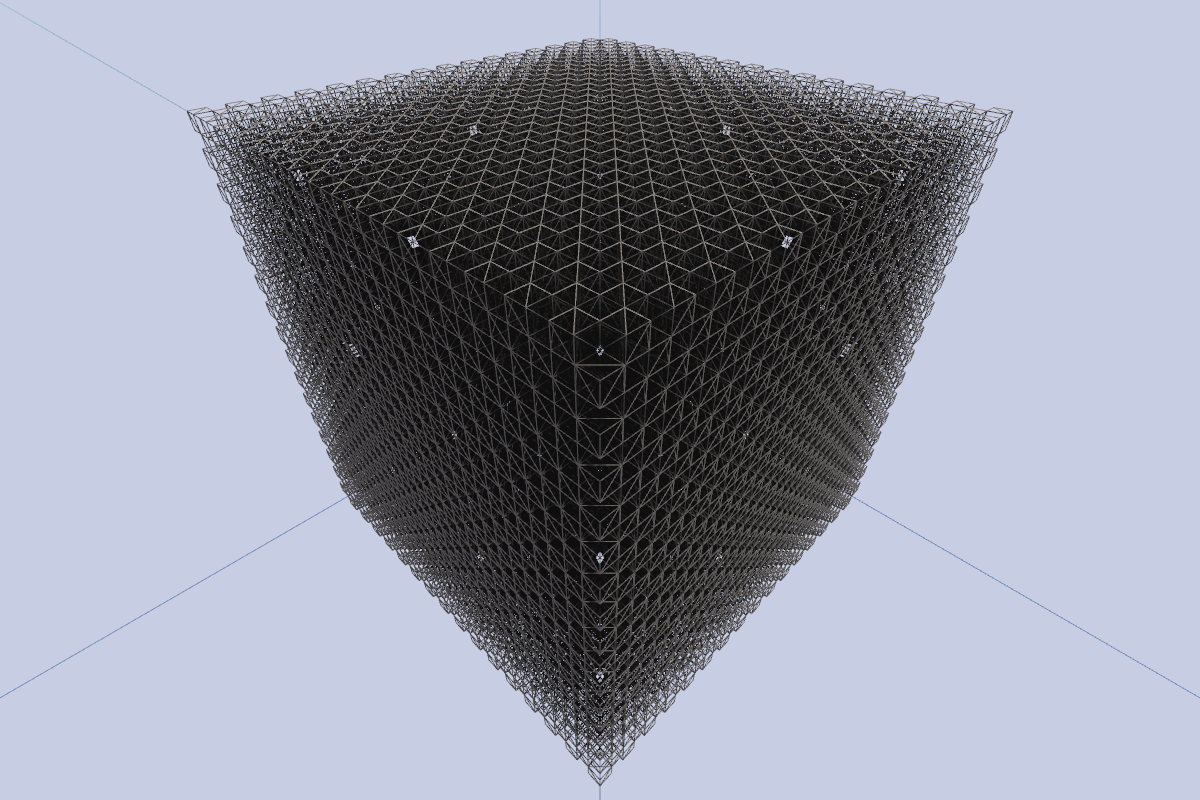
\includegraphics[width=.8\textwidth]{fps-cube.png}
	\caption{}\label{fig:cube}
\end{figure}
